\documentclass[11pt]{article}
\usepackage{fec}
\usepackage{mathtools}
\usepackage{longtable}
\usepackage{array}
\usepackage{graphicx}
\usepackage{lscape}
\usepackage{verbatim}
\usepackage{amsmath}
\usepackage{hhline}
\usepackage{subfigure}

\usepackage[dvipsnames]{xcolor}
\colorlet{LightRubineRed}{RubineRed!70!}
\colorlet{Mycolor1}{red}
\definecolor{Mycolor2}{HTML}{00F9DE}

\begin{document}
\newtheorem{theorem}{Theorem}
\newtheorem{corollary}{Corollary}
\newtheorem{lemma}{Lemma}
\newtheorem{definition}{Definition}
\DeclarePairedDelimiter{\norm}{\lVert}{\rVert} 

\title{Complexity of Pivot Algorithms}
\author{Qi Wang, Sean Kelley}
\date{December, 2020}
\maketitle


\begin{abstract}
Abstract...
\end{abstract}


\section{Introduction}
The Simplex method was invented by Dantzig in 1947 \cite{dantzig1951maximization} to solve the Linear Programming (LP) problem. It was a tableau based method which pivots between solutions under certain pivoting rules. Another framework of pivot algorithms is the criss-cross method, which was proposed by Zionts at 1969 \cite{fukuda1997criss} and then \cite{terlaky1987finite}, \cite{chang1979least} present a finite criss-cross version developed independently around 1980s. 

Many pivot rules have been designed, the result of which is that the simplex method and criss-cross have many variants depending on which pivot rule they employ. Some pivot rules have same motivation of Dantzig's original pivoting rule, which is to find a "best possible" nonbasis variable enter the basis, but these rules could cause cycling when the problem is degenerate (when some rhs coefficients of $b$ are zero). Thus a series pivot rules were proposed to ensure the algorithms are finite. Bland's rule is one of the them. We will present it and several other pivot rules in section \ref{secpivotrules}.

Csizmadia and Illés in 2010 \cite{csizmadia2012s} proved that a general pivot rule - the s-monotone index selection rule, which include Bland's, and two other index selection rules - can ensure the algorithms are finite. They also provide guidance towards revising other pivot rules to be finite. We present their research in section \ref{secsmono}. 

Although simplex method was generally efficient in practice, theoretically, Klee and Minty \cite{wikipediacontributors_2020_kleeminty} in 1970s showed the worst case complexity could happen. For a specific type of LP with $n$ variables and $n$ constraints, using the simplex method with Dantzig's rule, the number of iterations is $2^n-1$. We will demonstrate this in section \ref{secworst}.

Kitahara and Mizuno in 2011 \cite{kitahara2013bound} analyzed the complexity of the simplex method with certain pivot rules. They came up with a bound that is a polynomial of $n, m$, and special ratio. Such ratio is some constant in certain LO problems, such as when $A$ is unimodular and $b$ is integral. We showed their analysis \ref{seckita}.

\section{Notations}
In this paper, we consider the primal Linear optimization (LO) problem of the standard form
\begin{align}
\begin{split}
\min_x \quad &c^Tx\\
\text{s.t.} \quad &Ax = b\\
&x \ge 0\\
 x \in \Rmbb^n,\ c \in \Rmbb^n,\ &A \in \Rmbb^{m\times n},\ b \in \Rmbb^m   
\end{split} \label{LOprimal}
\end{align}
Table \ref{tbnotation} lists notations we will refer in the following part.
\begin{table}[h]
\caption{Notation}
\label{tbnotation}
\centering
\begin{tabular}{lll}
\hline
$n$ & number of variables   &  \\
$m$ & number of constraints (assume $m \le n$) &  \\
$B$ & set of index of basis solution $x_B$, $|B| = m$&  \\
$N$ & set of index of nonbasis solution $x_N$, $|N| = n-m$&  \\
\hline
\end{tabular}
\end{table}

\section{Pivot algorithms and pivot rules}
As we will go on to see in this article, much of our conversation will revolve around advancements in pivoting rules that led to performance increases for pivot algorithms. Before getting there, however, we would like to begin by discussing a few key improvements to other aspects of pivot algorithms that contributed to research focus in this space. We will start by going all the way back to the beginning.

\subsection{Dantzig's Simplex Algorithm}
As mentioned in our opening, the major advancement that opened the space of pivot algorithms was the development of the Primal Simplex Algorithm (referred to hereon as Simplex) by Dantzig, and his work will serve as our baseline for the complexity of pivot algorithms as we go on to compare them moving forward. In order to understand the complexity of the algorithm Dantzig proposed, let's take a moment to refresh ourselves on its operations. Although mentioned in greater detail in \cite{dantzig1951maximization}, the important details to recall are as follows. We begin by setting up the following system of equations where the equality exists between the first and second columns:
\[\begin{array}{|c|c|c|c|}
	\hline
	0 & -c_B^T x_B & -c_N^T x_N & x_0 \\
	\hline
	&&&\\
	b & A_B x_B & A_N x_N & 0 \\
	&&&\\
	\hline
\end{array}\]
Then with a couple of algebraic operations, we get the following tableau:
\[\begin{array}{|c|c|c|c|}
	\hline
	c_B^T A_B^{-1} b & 0 & (c_B^T A_B^{-1} A_N -c_N)^T x_N & x_0 \\
	\hline
	&&&\\
	A_B^{-1}b & Ix_B & A_B^{-1}A_N x_N & 0 \\
	&&&\\
	\hline
\end{array}\]

Simplex tells us to then pivot through bases until we find one that is either optimal or inconsistent. The pivoting operation for primal simplex method is as following
\begin{itemize}
	\item If there is dual infeasible
	\begin{itemize}
		\item Find a index from nonbasis, which are dual infeasible, i.e, choose $q \in \Qcal$ where $\Qcal
		:= \{j \in N: (c_B^T A_B^{-1} A_j -c_j) > 0\}$. If $|\Qcal| = 1$, we just choose the only index, otherwise we make choice by some rules (we talk later). 
		\item Find a index from basis by ratio test to keep the primal solution being feasible, i.e., choose $p \in \Pcal$ where $\Pcal:=\{\arg \min_{i \in B} \frac{x_i}{(A_B^{-1}A_q)_{i}}: (A_B^{-1}A_q)_{i} >0 \}$.  If $|\Pcal| = 0$, the LO is dual infeasible and primal unbounded, else if $|\Pcal| = 1$, we choose the only index, otherwise we make choice by some rules. 
		\item Perform a pivot: $B:= B \cup \{q\} \backslash \{p\}$, $N:= N \cup \{p\} \backslash \{q\}$.
	\end{itemize}
	\item else, the current solution solves the LO problem.
\end{itemize} 
\subsection{Criss-cross algorithm}
The difference between the criss-cross algorithm and simplex method is that criss-cross does not maintain either primal or dual feasibility, and thus omit the ratio test procedure. The similarities is that both simplex method and criss-cross algorithm are pivot algorithms and need some rules to choose the pivot element in each iteration. Such rule is crucial for the complexity and the finiteness of the whole algorithms. 
 
\subsection{Pivoting rules} \label{secpivotrules}
From now on, we focus on the simplex method unless otherwise stated. In simplex method, the decision of which nonbasis enter and which basis leaves (if more than one basis satisfy ratio test), is flexible. Thus many pivot rules are designed and we show some of them. 
\subsubsection{Dantzig's rule}
To make a pivot, Dantzig said to do the following:
\begin{itemize}
	\item Find the most positive element in the top row. Denote its index as $q$ ($n-m$ operations)
	\item Find the smallest $x_i/ \tau_{iq} : \tau_{iq} > 0$, where $\tau_{iq}$ is the $i$th element of the $q$th column in our tableau. If there is a tie, arbitrarily pick one of the tying elements ($3m$ operations)
	\item Swap $i$ and $q$ in their respective index sets.
	\item Multiply $A_B^{-1}$ by $A_N$ ($m^2*(n-m)$ operations)
	\item Add $c_B^T A_B^{-1} A_N$ to $-c_N^T$ ($m^2 + m(n-m) + (n-m)$ operations)
\end{itemize}
We see then this takes us to a total of $m^2 (n - m) + m^2 + m (n - m) + m + 2 n = O(m^2n)$ operations for the pivot.

Now as we showed in class \cite{class}, we know that so long as there is no degeneracy in the problem, simplex cannot cycle, so the number of pivots is bounded by the number of possible bases, which was $\binom{n}{m}$. Therefore, we know Dantzig's version of simplex to have complexity $O(\binom{n}{m}m^2n)$ for nondegenerate problems.

\subsubsection{Bland's Rule (Least-index)}
Now for Dantzig's simplex, we assumed that a problem would have no degeneracy, which is a rather high standard for using the algorithm in practice. To further complicate the matter, degeneracy leads to cycling in that version of simplex, which means the algorithm could run infinitely and never converge. To get around that issue then, many pivot rules have been proposed which help simplex avoid cycles. Arguably none of these such pivoting rules are more famous than Bland's Rule, which updates the above steps of simplex in the following way:
\begin{itemize}
	\item instead of picking the most positive top row element to enter the basis, pick the first positive top row element.
	\item instead of arbitrarily selecting a basis row matching the minimal ratio, select the minimal ratio basis row with least index.
\end{itemize}
As shown in \cite{bland}, these updates to Dantzig's simplex method ensure that we never cycle and make all linear programs converge and finite. Thus all linear programs now have complexity $O(\binom{n}{m}m^2n)$.

\subsubsection{Revised Simplex Method}
With simplex having a finite worst case across all problems, it is worthwhile to look at ways now to lower that upper bound. One of the first places the optimization community had success in doing this was with speeding up the process of making a pivot, which has come to be known as the Revised Simplex Method. Again, Revised Simplex differs from Dantzig's Simplex in two key ways \cite{revised}:
\begin{itemize}
	\item instead of calculating all of the objective row for each pivot, just calculate enough columns until we get a positive entry, pivoting on that (up to $n-m$ operations)
	\item instead of multiplying $A_B^{-1}$ by all of $A_N$, just multiply by the column corresponding to our first found positive entry ($m^2$ operations).
\end{itemize}
It is worth highlighting at this point that \cite{revised} shows Revised Simplex yields the same solution as Dantzig's Simplex but saves us from making many unnecessary calculations. This change brings our pivot to $2 m^2 + m (n - m) + m + 2 n = O(mn)$ operations (the same as in Dantzig's Simplex but swap $m^2(n-m)$ for $m^2$).


\subsubsection{Best improvement rule}

Also called largest improvement rule and greatest improvement rule. It aims for largest increase in objective value. It will pick the nonbasic variable with the $j := \arg \max_{j\in N}(c_B^T A_B^{-1} A_j - c_j)\times t_j$ where $t_j = \min_{i \in \{B:(A_B^{-1}A_j)_{i} >0\}} \frac{x_i}{(A_B^{-1}A_j)_{i}}$. In other words, the improvement to objective value is the reduced cost times the ratio. And we choose nonbasis that bring largest improvement in this iteration. For example, as in \cite{largest}, the tableau is
\begin{table}[h]
\centering
\begin{tabular}{cccccc}
                        & rhs                    & $-s_1$ & $-s_2$ & $-s_3$ & $-s_4$                    \\ \cline{2-6} 
\multicolumn{1}{l|}{$z$}  & \multicolumn{1}{l|}{0} & 2   & 3   & 0   & \multicolumn{1}{l|}{0} \\ \cline{2-6} 
\multicolumn{1}{l|}{$x_3$} & \multicolumn{1}{l|}{2} & 1   & 2   & 1   & \multicolumn{1}{l|}{0} \\
\multicolumn{1}{l|}{$x_4$} & \multicolumn{1}{l|}{3} & 1   & -1  & 0   & \multicolumn{1}{l|}{1} \\ \cline{2-6} 
\end{tabular}
\end{table}

Now $x_1, x_2$ are nonbasis that are dual infeasible. For $x_1$ we can increase it to $t_1 = \min \{\frac{2}{1}, \frac{3}{1}\} = 2$; for $x_2$, $t_2 = \min \{\frac{2}{2}\} = 1$. Since $2t_1 = 4 > 3 = 3t_2$, we choose $x_1$ to enter according to this rule.

Apparently, this rule need more arithmetic operations in each iteration. But it may save number of iterations, which we will talk later.

\subsubsection{Steepest edge rule}
Similar to Dantzig's rule, but instead of choose the most positive element in the top row, we choose $\max_{j \in N} \frac{c_B^TA_B^{-1}A_j - c_j}{\norm{A_B^{-1}A_j}}$ (normalize reduced cost with the norm of its column).

\subsubsection{Last-in-first-out rule (LIFO)}
Apart from Bland's rule, this last-in-first-out, plus the following most-often-selected-variable (MOSV) rule are also finite pivot rules. LIFO and MOSV are proposed by Zhang in 1997 \cite{zhang1999new}. LIFO means among the candidates, choose the most recently moved variable. In the first iteration with no selection in the past, we use Bland's rule or Dantzig's rule.

\subsubsection{Most-often-selected-variable (MOSV)}
MOSV rule is to select the variable that has been selected the largest amount of times before, that is the "most often selected". In the first iteration with no selection in the past, we use Bland's rule or Dantzig's rule.

Also, when choice by LIFO (or MOSV) rule is not unique, we use Dantzig's rule. This called Hybrid-LIFO (Hybrid-MOSV) \cite{zhang1999new}.

\subsection{S-monotone index selection rules} \label{secsmono}
Csizmadia and Illés in 2010 \cite{csizmadia2012s} proposed that Bland, LIFO, MOSV pivot rules are s-monotone index selection rules. They provide a explicit definition of s-monotone index selection rules in \cite{csizmadia2012s}. The key steps of s-monotone rule are
\begin{enumerate}
\item Maintain a sequence of vectors $s_k \in \Ncal^n$, where $k$ is the iteration number. 
\item At iteration $k$, when selecting index from a couple of candidates (tie in entering or leaving), select the index $j := \arg \max_j s_k^j$, where $j$ is the index of $s_k$.
\item When finishing pivoting, generate $s_{k+1}$ by $s_{k}$ and specific rules for Bland, LIFO and MOSV (we talk latter). 
\item $s_k$ is an nondecreasing vector from $k=0,1,2,\cdots$.
\end{enumerate}
We define $i_k, o_k$ are indices of entering variable and leaving variable at iteration $k$. The $s_k$ for Bland, LIFO, MOSV is generated as follows

\begin{itemize}
\item \textbf{Bland}. $s_k = (n, n-1, \cdots, 1)^T$ for all $k$.
\item \textbf{LIFO}. \begin{align*}
s_{k+1}^i = \left\{
\begin{aligned}
&k, & \text{if } i \in \{i_k, o_k\},\\
&s_k^i & \text{ otherwise}. 
\end{aligned}
\right.
\end{align*}
\item \textbf{MOSV}. \begin{align*}
s_{k+1}^i = \left\{
\begin{aligned}
&s_k^{i} + 1, & \text{if } i \in \{i_k, o_k\},\\
&s_k^i & \text{ otherwise}. 
\end{aligned}
\right.
\end{align*}

\end{itemize}
Csizmadia and Illés \cite{csizmadia2012s} then proved simplex method (as well as criss-cross) with s-monotone rule is finite algorithm. They also provided guidance of revising other pivot rules to be finite. For example, if we want to apply steepest edge rule but want to be finite, we can make some modification that, 
\begin{enumerate}
\item At the beginning, define a sequence $\{p_k\}$ that is strictly increasing.
\item At iteration $k$, let
$$
\gamma = \max_{j \in N} \frac{c_{B^k}^TA_{B^k}^{-1}A_j - c_j}{\norm{A_{B^k}^{-1}A_j}},
$$
and adjust $p_k$ by
 \begin{align*}
p_k = \left\{
\begin{aligned}
&p_k + \delta, & \text{if } p_{k-1} \ge \gamma,\\
&\gamma, & \text{ otherwise}. 
\end{aligned}
\right.
\end{align*}
where $\delta > 0$ is a given number. The $\{p_k\}$ by such adjustment is strictly increasing. Therefore we can use it to update the $s_{k}$ as follows (similar to LIFO)
\begin{align*}
s_{k}^i = \left\{
\begin{aligned}
&p_k, & \text{if } i \in \{i_k, o_k\},\\
&s_{k-1}^i & \text{ otherwise}. 
\end{aligned}
\right.
\end{align*}
\item Select the candidates (of indices) that has largest value of $s_k$.
\end{enumerate}
In such way the steepest edge method is combined with LIFO, and is s-monotone index rules (finite). It can also be combined with MOSV similarly. Consequently, they state an possible research direction is that to analyze the complexity of s-monotone index selection rules.

\section{Contemporary complexity analysis}
\subsection{When will worst case happen} \label{secworst}
Given $m$ constraints and $n$ variables, there are at most $\binom{n}{m}$ possible basis. When $m=\frac{n}{2}$, $\binom{n}{m}$ get its maximum $\binom{n}{\frac{n}{2}}\approx \sqrt{\frac{2}{\pi n}}2^n$,  which is the worst complexity. Klee and Minty defined a type of LO problems that primal simplex with Dantzig's rule may visit all vertices before finally finding the optimal solution. Detailed introduction of Klee Minty cube can be referred to \cite{vanderbei2020linear}. Here we demonstrate some examples. Klee Minty cube is defined as following LO problem \ref{eq:klLO}. The coefficients might be different in other articles. 
\begin{align}
\begin{split}
\max &\sum_{j=1}^n 2^{n-j}x_j \\
\text{s.t. } & 2\sum_{j=1}^{i-1}2^{i-j}x_j + x_i \le 5^i, \quad i=1,\cdots,n\\
			&x_j \ge 0,  \quad j=1,\cdots,n
\end{split}\label{eq:klLO}
\end{align} 
When $n=2$ and $n=3$ the 2-d and 3-d Klee Minty LO problems are 
\begin{align*}
\begin{split}
\max \quad & 2x_1 + x_2 \\
\text{s.t. }\quad  & x_1 \le 5\\
& 4x_1 + x_2 \le 25\\
& x_1 \ge 0,\ x_2 \ge 0.
\end{split}
\begin{split}
\max \quad & 4x_1 + 2x_2 + x_3 \\
\text{s.t. }\quad  & x_1 \le 5\\
& 4x_1 + x_2 \le 25\\
& 8x_1 + 4x_2 + x_3 \le 125\\
& x_1 \ge 0,\ x_2 \ge 0, \ x_3 \ge 0.
\end{split}
\end{align*}
The feasible region of 2-d and 3-d Klee Minty problems are shown in Figure \ref{fig:kmcube}. They look like "squashed" square and cube.
\begin{figure}
    \centering
    \subfigure[]{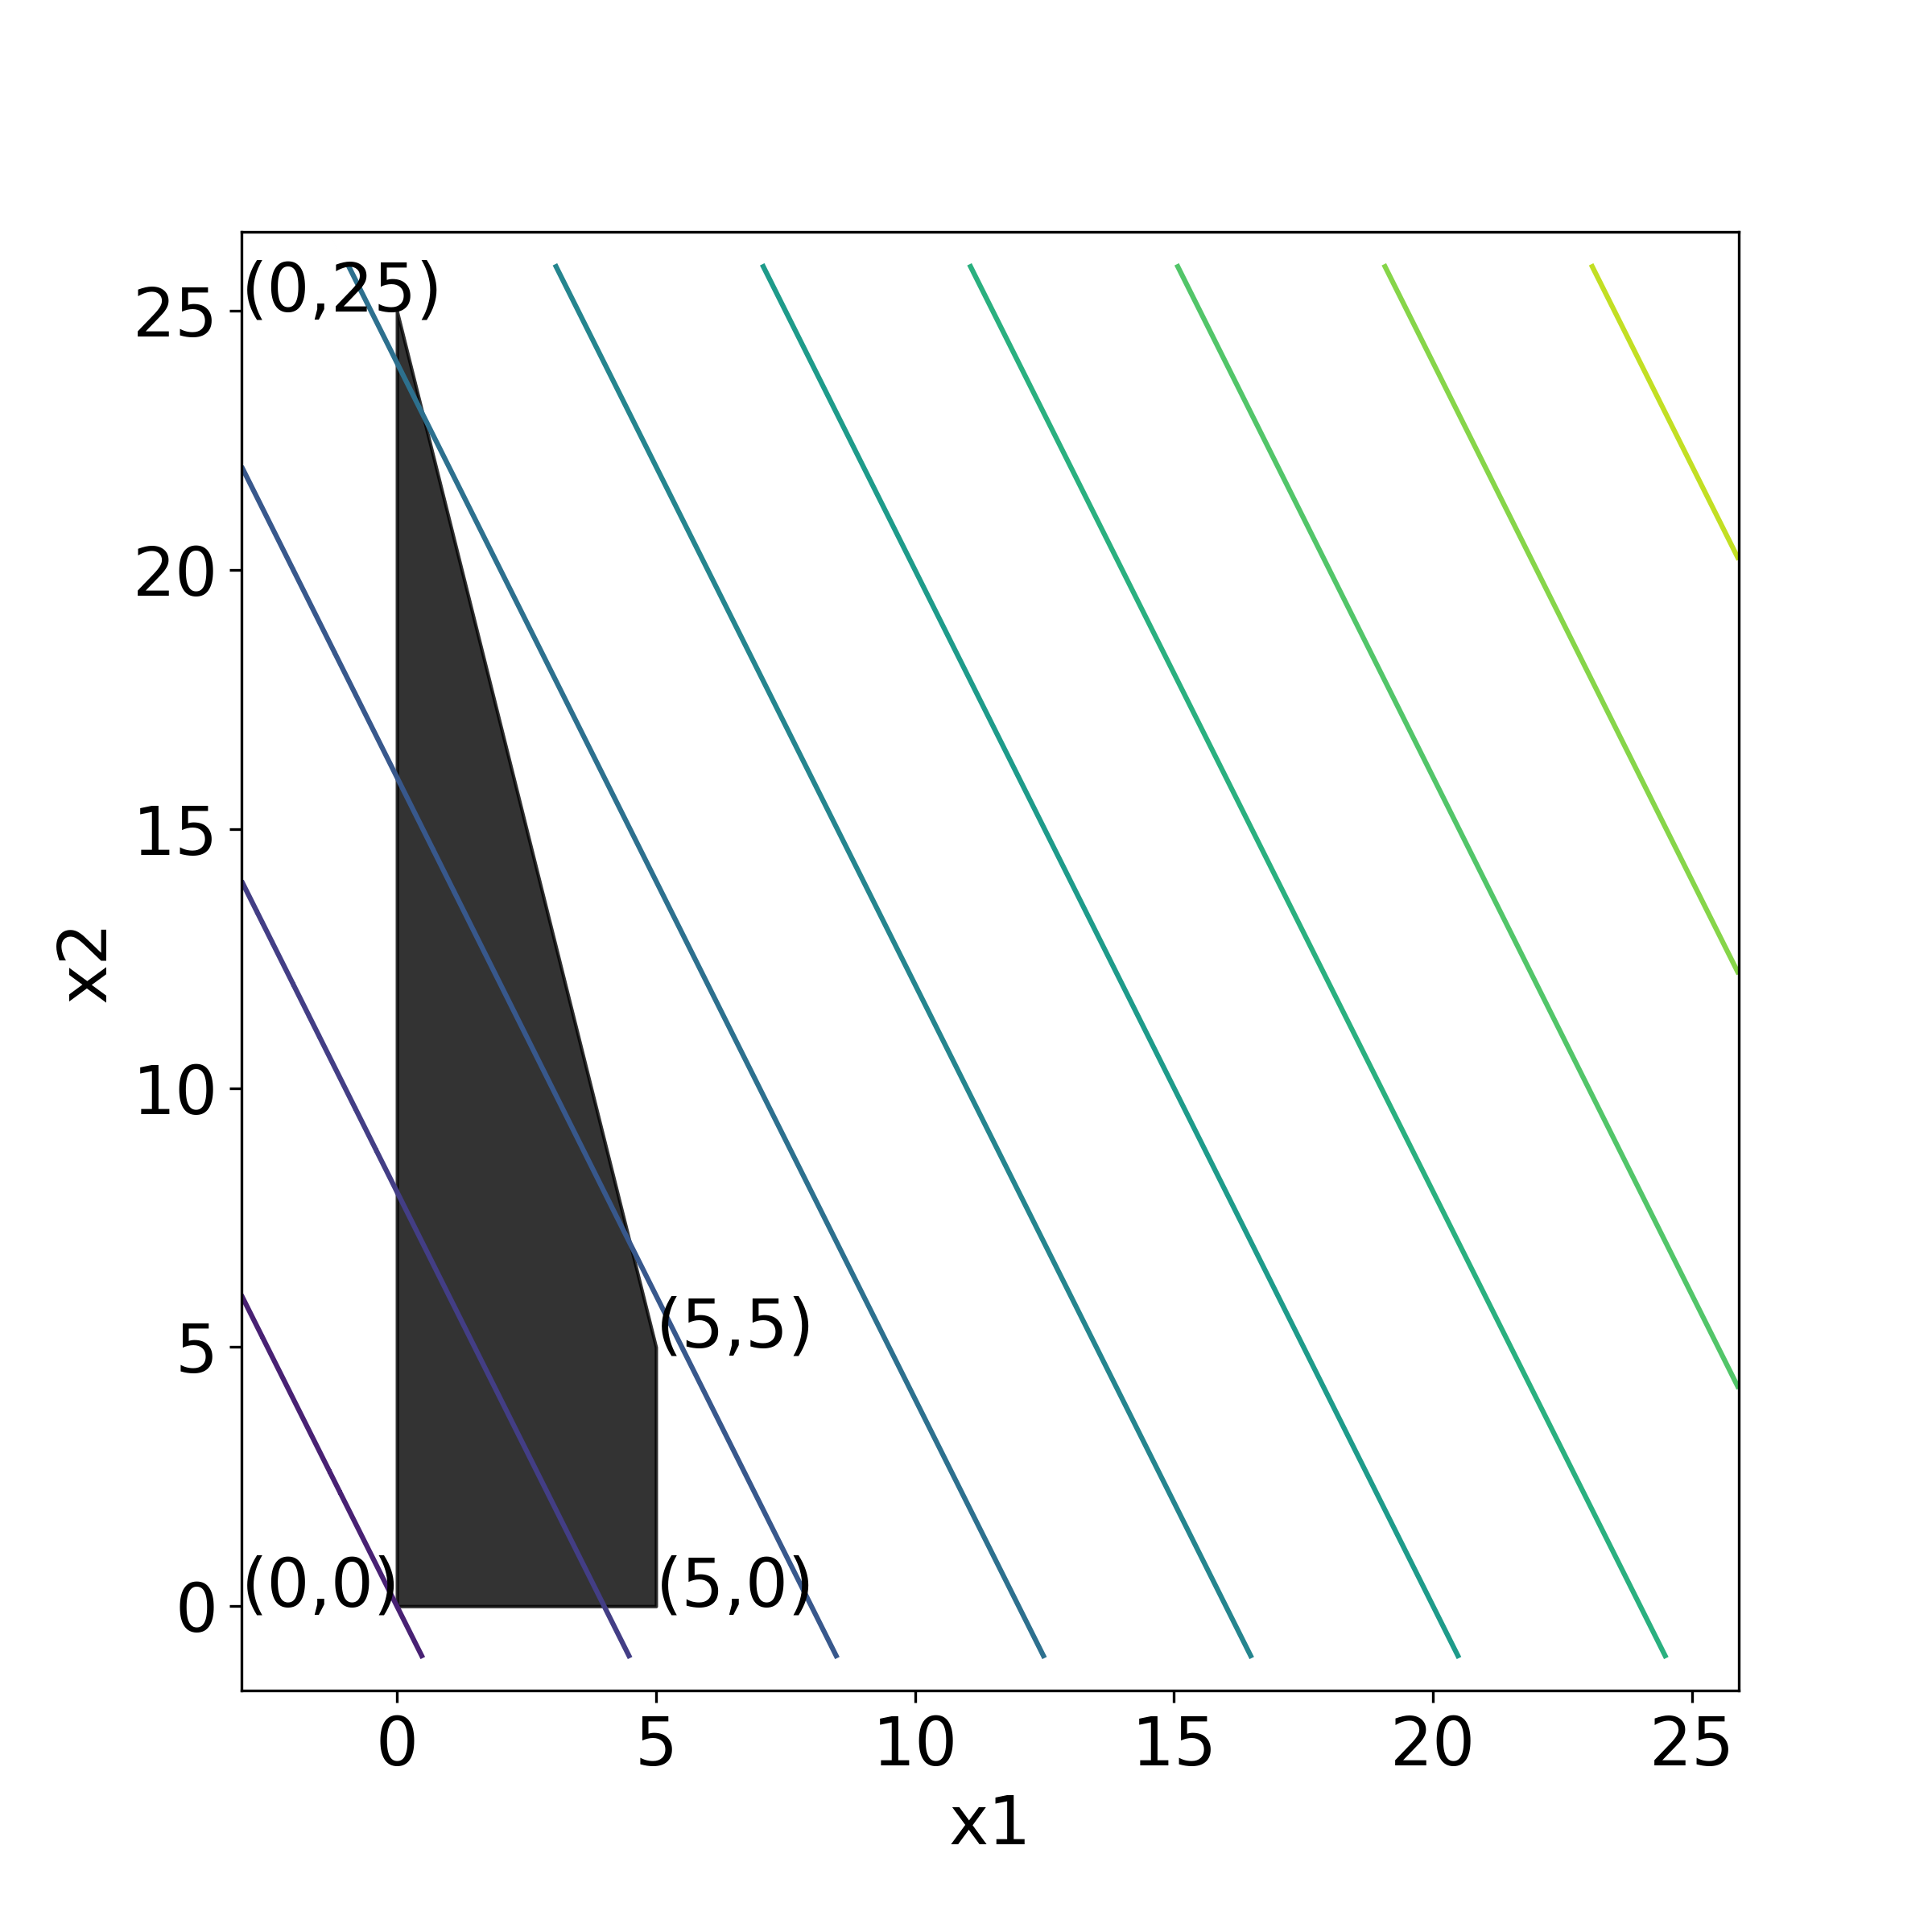
\includegraphics[width=0.38\textwidth]{klee_cube_d2.png}}
    \subfigure[]{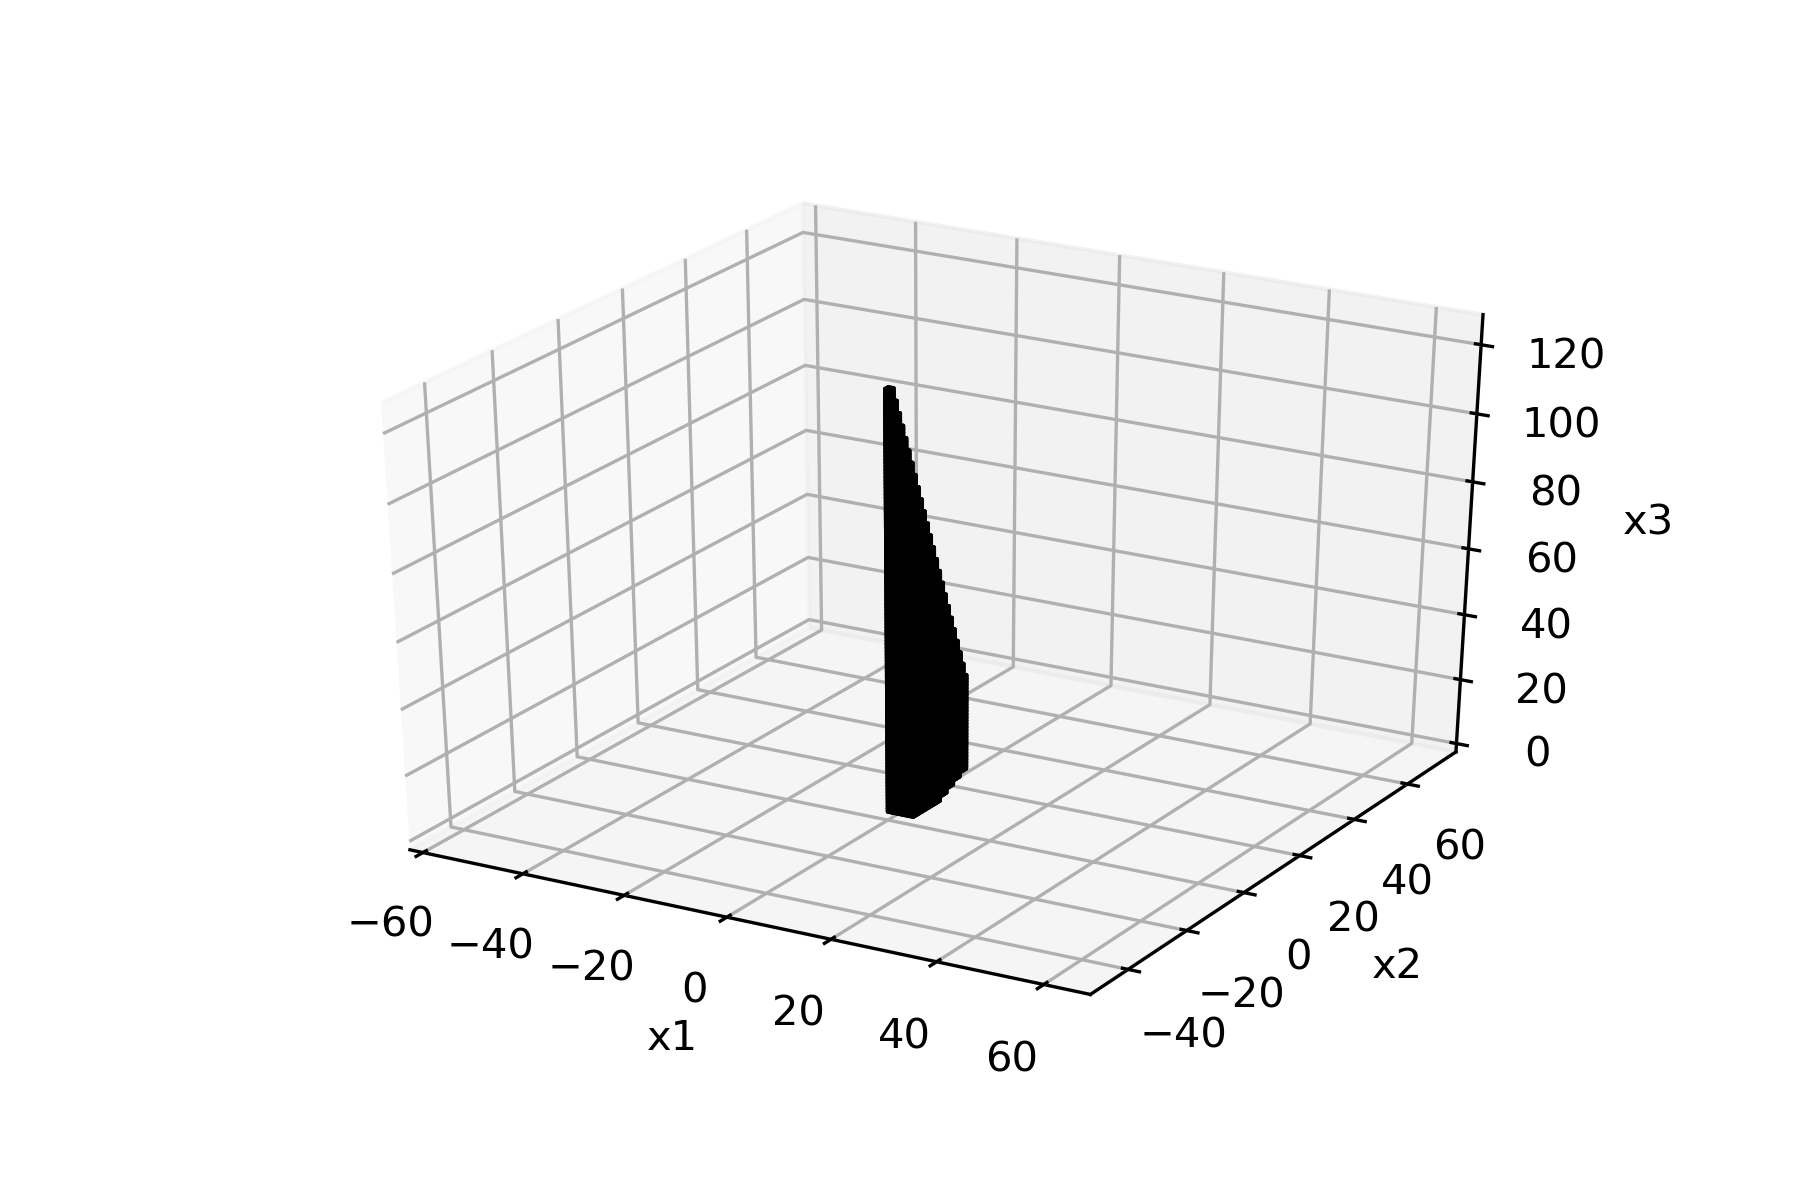
\includegraphics[width=0.59\textwidth]{klee_cube_d3.png}}
    \caption{(a) Feasible region of 2-d Klee Minty Cube with contour lines (b) Feasible region of 3-d Klee Minty Cube}
    \label{fig:kmcube}
\end{figure}
We apply primal simplex method (a) least-index and (b) Dantzig pivot rules to demonstrate the number of iterations. Table \ref{Table: tableau} shows the tableau of least-index primal simplex method. Dantzig's rule coincides with result of least-index rule in this example. 

\begin{table}[H]
\caption{Tableau of primal simplex method (least index version), the element with * is the pivot element. }
\label{Table: tableau}
\centering
\begin{tabular}{c|llllll}
   & rhs & $x_1$ & $x_2$ & $s_1$ & $s_2$ &                 \\ \cline{1-6}
$z$  & 0   & 2  & 1  & 0  & 0  & at vetex (0,0)  \\
$s_1$ & 5   & $1^*$  & 0  & 1  & 0  &                 \\
$s_2$ & 25  & 4  & 1  & 0  & 1  &                 \\ \hhline{======}
$z$  & -10 & 0  & 1  & -2 & 0  & at vetex (5,0)  \\
$x_1$ & 5   & 1  & 0  & 1  & 0  &                 \\
$s_2$ & 5   & 0  & $1^*$  & -4 & 1  &                 \\ \hhline{======}
$z$  & -15 & 0  & 0  & 2  & -1 & at vetex (5,5)  \\
$x_1$ & 5   & 1  & 0  & $1^*$  & 0  &                 \\
$x_2$ & 5   & 0  & 1  & -4 & 1  &                 \\ \hhline{======}
$z$  & -25 & -2 & 0  & 0  & -1 & at vetex (0,25) \\
$s_1$ & 5   & 1  & 0  & 1  & 0  &                 \\
$x_2$ & 25  & 4  & 1  & 0  & 1  &                 \\ \hhline{======}
\end{tabular}
\end{table}
By taking a look at the constraints, the first constraint says that $x_1 \le 5$. The second constraint says that $x_2 \le 25$ and $x_2$ is smaller depending on how big $x_1$ is. Similarly, the third constraint says that $x_3 \le 125$ (again, smaller depending on $x_1$ and $x_2$). Therefore, the constraints are approximately a set of upper bounds, which means that the feasible region is virtually a stretched n-dimensional hypercube with $2^n$ vertices. For such problem, primal simplex method with Dantzig's rule will iterate $2^n -1$ pivot steps.

\subsection{Kitahara and Mizuno analysis} \label{seckita}
In 2011, Kitahara and Mizuno \cite{kitahara2013bound} proved the complexity can be bounded by a polynomial of $m, n$ and a special ratio. They utilized the analysis of Ye (2010) \cite{ye2010simplex} for Markov Decision Problem. We summarize the key results of Kitahara and Mizuno \cite{kitahara2013bound} in this section. 

We define some new notations. A BFS is said to be a basic feasible solution for primal LO problem (\ref{LOprimal}). Let $\delta$ and $\gamma$ be the minimum and the maximum values of all the positive elements of all BFSs. That is, for any BFS $\hat{x} \in \Rmbb^{n}$, if $\hat{x}_j \neq 0, \ j \in \{1, \cdots, n\}$ where the subscript $j$ represent the $j$th entry of $\hat{x}$, we have 
\begin{align}
\delta \le \hat{x}_j \le \gamma. \label{eq:bfsbound}
\end{align} 

The most important result of Kitahara and Mizuno \cite{kitahara2013bound} is the following theorem and corollary.
\begin{theorem}
When we apply the simplex method with the Dantzig's rule or the best improvement rule for LO \ref{LOprimal} having optimal solutions, we encounter at most
\begin{align}
n\lceil m \frac{\gamma}{\delta}\log(m\frac{\gamma}{\delta})\rceil \label{kmcomplexity}
\end{align}
different basic feasible solutions. \label{KTheorem1}
\end{theorem}

\begin{corollary}
 If the primal problem is nondegenerate, the simplex method finds an optimal solution in at most $n\lceil m \frac{\gamma}{\delta}\log(m\frac{\gamma}{\delta})\rceil$ iterations.
\end{corollary}

The proof can be referred to Kitahara and Mizuno \cite{kitahara2013bound}. Therefore the bound (\ref{kmcomplexity}) is a polynomial of $n, m$ and $\frac{\gamma}{\delta}$ with assumptions that the primal LO \ref{LOprimal} has optimal solutions and is nondegenerate. Therefore, for Klee-Minty problem \ref{eq:klLO}, $\gamma = 5^n$ while $\delta = 5$ and there ratio is exponential to $n$. This theoretically explains the complexity of Klee-Minty cube problem.

In practical, the ratio of $\frac{\gamma}{\delta}$ is not easy to get prior to solving the problem. However, for some specific LO, $\frac{\gamma}{\delta}$ can be bounded using LO coefficients. 
\subsubsection{LO with a totally unimodular matrix A and integral b}
\begin{definition}
A matrix A is totally unimodular if every square submatrix has determinant 0, -1 or 1. In particular, this implies that all entries are 0, -1 or 1.
\end{definition}
Totally unimodular matrices are very well behaved, because they always define polytopes with integer vertices, as long as the right-hand side is integer-valued. Many practical problem can be modelled using totally unimodular matrices, such as the node arc incidence matrix of a directed graph.

With totally unimodular $A$ and integral $b$, all the elements of any BFS are integers, so $\delta \ge 1$. And for a BFS $x = (x_B, x_N)$, $x_N = 0$ and $x_B = A_B^{-1}b \ge 0$, since $A_B$ is totally unimodular, $A_B^{-1}$ is unimodular \cite{kitahara2013bound} and all the elements of $A_B^{-1}$ are $-1, 0$ or $1$. Thus for any $j \in B$ we have $x_j \le \norm{b}_1$, which implies $\gamma \le \norm{b}_1$. Thus $\frac{\gamma}{\delta} \le \frac{\norm{b}_1}{1}$. Thus by Theorem \ref{KTheorem1}, we have
\begin{corollary}
Assume that the constraint matrix A of LO (\ref{LOprimal}) is totally unimodular and the constraint vector b is integral. When we apply the simplex method with the Dantzig's rule or the best improvement rule for LO (\ref{LOprimal}), we encounter at most $n\lceil m \norm{b}_1\log(m\norm{b}_1)\rceil$ different basic feasible solutions. Moreover if the LO (\ref{LOprimal}) is nondegenerate, this is the most iterations to find optimal solution. 
\end{corollary}

%\section{title}
%There are certain pivot rules:
%\begin{itemize}
%\item Bland's rule, lexicographic rule
%\item Clairvoyant pivot rule (only theoretical), unimplementable
%\item Hirsch conjecture : disproven by Francisco Santos, 2011
%\item Polynomial Hirsch conjecture -- still open
%\end{itemize}

\subsection{Del Pia and Michini Analysis}
Earlier this year, another paper was released by Del Pia and Michini further refining the upper bounds on required pivots to solve certain subclasses of linear programs \cite{pia}. In their case, they focus on the simplex paths for LP's defined over lattice polytopes (i.e. polytopes with only integer vertices). Their analysis of these paths hinge on the following four algorithms.

\subsubsection{Algorithm Review and Complexity}
\begin{itemize}
	\item A Basic Algorithm (A simplex method that avoids cycling) \\
	\textbf{Input}: Lattice Polytope $P$, vector $c$, vertex $x^0$ of $P$ \\
	\textbf{Ouput}: Vertex $x^*$ maximizing $P$ 

	\item A Scaling Algorithm \\
	\textbf{Input}: Lattice Polytope $P$, vector $c$, vertex $x^0$ of $P$ \\
	\textbf{Ouput}: Vertex $x^*$ maximizing $P$
	\begin{enumerate}
		\item Let $l = \lceil \text{log}\Vert c \Vert_\infty \rceil$. Define approximations $c^i = \lceil c/2^{l - i} \rceil$.
		\item For $i \in [l]$, let $x^{i+1} = \text{Basic Algorithm}(P, c^i, x^i)$.
		\item Return $x^{l+1}$ optimal.
	\end{enumerate}
	\item A Preprocessing and Scaling Algorithm \\
	\textbf{Input}: Lattice Polytope $P$, vector $c$, vertex $x^0$ of $P$ \\
	\textbf{Ouput}: Vertex $x^*$ maximizing $P$
	\begin{enumerate}
		\item Perturb $c$ as described in Section 3 of \cite{preprocess}. Denote the output as $\bar{c}$
		\item Let $x^* = \text{Scaling Algorithm}(P, \bar{c}, x)$
		\item Return $x^*$ optimal.
	\end{enumerate}
	\item An Iterative Scaling Algorithm \\
	\textbf{Input}: Lattice Polytope $P$, vector $c$, vertex $x^0$ of $P$ \\
	\textbf{Ouput}: Vertex $x^*$ maximizing $P$
	\begin{enumerate}
		\item Let $x^* = x^0$.
		\item Let $\bar{c}$ be projection of $c$ onto one active constraint from each previous iteration. If $\bar{c} = 0$, return $x^*$
		\item Let $\tilde{c}$ be the perturbation of $\bar{c}$ as described in Section 4 of \cite{pia}.
		\item Let $x^* = \text{Scaling Algorithm}(P, \tilde{c}, x^*)$. Return to 2.
	\end{enumerate}
\end{itemize}

With these four algorithms, Del Pia and Michini go on to prove the following results.
\begin{itemize}
	\item Basic Algorithm length $\leq nk \Vert c \Vert_\infty$
	\item Scaling Algorithm length is $O(nk \text{ log}\Vert c \Vert_\infty)$
	\begin{itemize}
		\item Basic Algorithm is called $\text{log}\Vert c \Vert_\infty) + 1$ times.
		\item For scaled $c$ each run of Basic Algorithm has $\leq nk$ pivots.
	\end{itemize}
	\item Preprocessing and Scaling Algorithm length is $O(n^4k \text{ log } nk))$
	\begin{itemize}
		\item Perturbed $c$ reduces the number of times the Scaling Algorithm has to call the Basic Algorithm from $\text{log} \Vert c \Vert_\infty$ to $n^3 \text{ log } nk$.
		\item For each scaling of perturbed $c$, the run of Basic Algorithm still has $\leq nk$ pivots.
	\end{itemize}
	\item Iterative Scaling Algorithm length is $O(n^2 k \text{ log } nk\alpha)$, where $\alpha$ is the largest element in $A$.
	\begin{itemize}
		\item Iterative Scaling Algorithm has at most $n$ iterations.
		\item The perturbation of $\bar{c}$ makes $\Vert \tilde{c} \Vert_\infty \leq n^3 k \alpha$.
		\item Recall that the Scaling Algorithm's length is $O(nk \text{ log}\Vert \tilde{c} \Vert_\infty)$, which in this case becomes $O(nk \text{ log } n k \alpha)$
	\end{itemize}
\end{itemize}
Furthermore, for each algorithm, the authors show for a given set of inputs that the solution is the same as if those inputs had been run directly against simplex.

Now when looking at the last two results above, we appear to see a polynomial complexity for solving a problem with simplex (since we showed pivot calculations earlier to be polynomial). Now at first glance this might be exciting, but let's take a moment to recall their hypothesis. Del Pia and Michini assume our feasible vertices form a lattice polytope, which can rule out many LP's. Additionally, they state that the complexity is in terms of the number of vertices simplex visits, which in the case of a problem with degeneracy, is not the same as the number of pivots. So although this complexity, as we'll see next, is a nice improvement over the previous case of solving this class of LP, this class is a rather small subspace of all LP's. This isn't to say this work is insignificant, however, as much as it is to say there would be great value in further research to generalize this method to solve a wider variety of problems.

\subsection{Relationship to Previously Discussed Works}
The work of Del Pia and Michini builds on and relates to multiple other topics in this paper, and we would like to take a moment now to call out some of the highlights. Most noticeably, at the base of all of the algorithms developed by Del Pia and Michini was their Basic Algorithm, which finds an optimal solution over a lattice polytope for a cost vector. At its core, this Basic Algorithm runs an arbitrary non-cycling simplex method, which could be any one of the pivot algorithms mentioned before this section.

The second comparison worth calling out is the relationship between this result and those of Kitahara. Although Del Pia and Michini do the work of their paper with a general form of an LP, they mapped their problem to standard form to compare it to Kitahara. After doing so, they proved for the case the problem exists in a [0,k] polytope that Kitahara's bound was exponential for the number of vertices in the simplex path, whereas shown above, their bound is polynomial. In the case we just consider an LP in a [0,1]-polytope (thus the results of Kitahara apply since we have unimodular $A$), Del Pia and Michini show Kitahara's upper bound to simplify to  $O(n^3 \text{ log } n)$ while theirs reduces to $O(n^2 \text{ log } n)$. We see then their result is a nice improvement in terms of complexity, and, since it applies to a wider array of problems, it is even much more general as well.

\subsection{Software Implementations}
After taking a bit of an account of the history of pivot algorithms, all the way from Dantzig to advances this year, we thought it may be of interest to the reader to point out what in our review is leveraged in practice. In his 2015 \cite{bixby} talk, Bob Bixby goes into detail the implementation details of Gurobi and Cplex. In the early parts of this paper, we find a lot of overlap with what is used. In both solvers we find implementations of primal simplex using revised simplex to calculate each pivot. He goes on to detail that for a pivoting rule both softwares use steepest-edge since computational experiments have shown it to both find short paths around the feasible region as well as paths that are easy to calculate. The surprising point in the talk was that neither software actually uses a pivot rule with an anti-cycling scheme, which led us to conclude many of our mentioned pivot rules are actually not that useful in practice. Instead, both softwares have a way of perturbing the problem (by adjusting lower bounds slightly) so that degeneracy goes away but yet we still end up with the same optimal solution. Since there were a recent advancement and theory not yet uncovered at the time of Bixby's talk, we decided to do a little outside searching for implementations of Del Pia's and Kitahara's papers. We were not able to find implementations for either, and we think this to be the case because the results are not general enough to be useful to LP solvers.

\section{Conclusion}

\bibliographystyle{plainurl}
\bibliography{reference.bib} 

\end{document}
